\chapter{Introducción específica}
\label{Chapter2}

En este capítulo se presentan en detalle las tecnologías y conceptos utilizados para el trabajo. Se parte de una introducción a las imágenes generadas por vehículos aéreos no tripulados (UAV), específicamente imágenes generadas por drones. Luego, se mencionan herramientas adicionales utilizadas en los procesos de soporte de proyectos orientados a IA, como lo son el proceso de etiquetado y la gestión de los datos. Finalmente, se puntualiza en modelos y métricas utilizados en VPC para este tipo de trabajos.

\section{Imágenes generadas por vehículos aéreos}
\label{sec:imgUAV}

Los UAV han emergido como herramientas fundamentales en la obtención de imágenes aéreas de alta resolución. Su empleo ha permitido avances significativos en diversos campos, entre los que se destacan la agricultura de precisión, la vigilancia ambiental y la inspección de infraestructuras, entre otros \citep{mokhtar_image_2023}.

La utilización de UAV en la adquisición de imágenes se fundamenta en varias ventajas inherentes a estos sistemas. En primer lugar, la flexibilidad operativa que ofrecen permite la planificación de vuelos adaptados a necesidades específicas de cada proyecto, garantizando la cobertura de zonas amplias o de difícil acceso (por ejemplo, palmeras en ubicaciones privadas de Montevideo o zonas en donde el acceso a pie es muy costoso). Asimismo, la capacidad de llevar equipamiento especializado (como cámaras multiespectrales, sensores térmicos y dispositivos LiDAR) posibilita la obtención de datos con distintos niveles de resolución y en diversas bandas del espectro electromagnético, lo cual es esencial para aplicaciones que requieren análisis detallados y precisos \citep{unmanned_system_technology_uavdrone_nodate}.

Otro aspecto relevante es la eficiencia en términos de tiempo y costos. Comparados con métodos tradicionales de monitoreo, los UAV reducen considerablemente los recursos necesarios para este tipo de tareas, al tiempo que minimizan la exposición de personal a ambientes potencialmente peligrosos. Esto, sumado a la posibilidad de repetir vuelos en condiciones controladas, favorece la generación de series temporales de datos que permiten, en conjunción con el monitoreo, el análisis evolutivo de fenómenos específicos (como lo son las plagas).

Los UAV (como los drones) suelen cubrir un área específica; sin embargo, los vuelos de aviones tripulados cubren un área mucho mayor \citep{2000_aviation_ortoimagenes_nodate}. El servicio de geomática de la IM utiliza estas dos tecnologías para generar imágenes de todo Montevideo. Cada dos o tres años se realiza un vuelo de avión que cubre toda la ciudad. En contraste, los vuelos de drones pueden ser solicitados a demanda, dado que su costo es mucho menor.

La diferencia entre estas tecnologías no solo radica en el costo y área cubierta, sino también en el tipo de cámara que llevan estos vehículos. La resolución espacial de las imágenes generadas dependen de la cámara y la altura a la que vuelan estos vehículos (estas imágenes son procesadas por varios software, uno de ellos es Agisoft \citep{agisoft_agisoft_nodate}, que permite generar los ortomosaicos).

\subsection{Imágenes de drones}
\label{sec:imgUavDrones}

Las imágenes generadas por drones se destacan por su alta resolución y capacidad para capturar detalles finos del terreno. Estas imágenes suelen tener una mayor resolución (medida en \si{\centi\meter\per\pixel}) en comparación con las generadas por aviones. El DJI Phantom 4 PRO \citep{dji_support_nodate} es ampliamente utilizado en aplicaciones de mapeo y fotogrametría debido a su capacidad para generar ortomosaicos con una resolución de hasta \SI{5}{\centi\meter\per\pixel} (volando a 100 metros de altura). Otro dron ampliamente utilizado es el DJI MAVIC 3 Enterprise RTK \citep{dji_specs_nodate}. La integración de tecnología RTK \citep{wikipedia_rtk_2024} en este dron permite una mayor precisión en la georreferenciación de las imágenes capturadas. A diferencia del DJI Phantom 4 PRO, que necesita puntos de apoyo relevados en el campo tomados con un GPS RTK (en las ejecuciones de vuelos con el DJI Phantom de la IM, los puntos de apoyo fueron tomados con GNSS SinoGNSS T300 Plus \citep{comnav_technology_ltd_receptor_nodate}, utilizando corrección en tiempo real por NTRIP \citep{wikipedia_networked_2025} con la base UYMO del Instituto Geográfico Militar uruguayo).

\section{Herramientas de soporte en utilizadas en IA}
\label{sec:herramSopIA}

La cara visible de los proyectos de inteligencia artificial se fundamenta, en general, en los resultados y aplicaciones derivados de modelos de aprendizaje automático. No obstante, al igual que en cualquier proyecto de software, resulta fundamental integrar buenas prácticas de ingeniería de software, lo que implica focalizarse en atributos específicos del sistema, tales como la escalabilidad, la seguridad y la recuperabilidad, entre otros \citep{sommerville_software_2015}. Para alcanzar estos objetivos, es crucial considerar disciplinas que faciliten su consecución, como la gestión de la configuración o la gestión de datos. A continuación, se exponen algunas herramientas de apoyo a varios de estos procesos.

\subsection{Gestión de código}

El control de versiones es fundamental para asegurar la trazabilidad en los proyectos. Git permite mantener un historial detallado de los cambios, facilitando la integración de nuevas funcionalidades y la resolución de conflictos mediante estrategias de \textit{branching} y \textit{merging}. Esta práctica no solo mejora la trazabilidad, sino que brinda transparencia y contribuye a la reproducibilidad del proyecto a lo largo del tiempo. Una de las implementaciones más conocidas es GitHub \citep{github_build_nodate}, la cual se ha consolidado como una plataforma de colaboración que posibilita la gestión distribuida de proyectos de software en entornos tanto académicos como empresariales.

\subsection{Gestión de infraestructura}

La correcta administración de la infraestructura es esencial para el despliegue y mantenimiento de aplicaciones de inteligencia artificial, tanto en entornos de desarrollo como en producción. Para ello, en la industria se suelen utilizar diversas herramientas, entre las cuales se encuentran:

\begin{itemize}
	\item Docker y Docker Compose \citep{merkel_docker_2014} \citep{docker_docker_0000}: estas herramientas permiten la creación de contenedores que encapsulan una aplicación (o varias aplicaciones) y sus dependencias, asegurando un entorno de ejecución uniforme y reproducible en diferentes sistemas. Docker Compose facilita la orquestación de múltiples contenedores, posibilitando la simulación de entornos complejos en local.
	\item Vagrant \citep{hashicorp_vagrant_2023} \citep{hashicorp_documentation_nodate}: se utiliza para la configuración y despliegue de máquinas virtuales. Esta herramienta ofrece un entorno virtualizado consistente y de fácil replicación, lo que resulta útil para la estandarización del entorno de desarrollo simplemente con un archivo de configuración (\textit{Vagrantfile}).
	\item OpenShift \citep{red_hat_openshift_2023} \citep{red_hat_red_nodate} y Helm \citep{the_helm_authors_helm_2023} \citep{the_helm_authors_docs_nodate}: en entornos de producción, OpenShift basado en Kubernetes \citep{wikipedia_kubernetes_2025}, permite una gestión centralizada y escalable de las aplicaciones, mientras que Helm simplifica la instalación, configuración y actualización de las mismas mediante el uso de paquetes predefinidos.
\end{itemize}

\subsection{Gestión de usuarios y permisos}

La seguridad y la privacidad son aspectos críticos en el desarrollo de aplicaciones de inteligencia artificial. La correcta gestión de usuarios y permisos es esencial para garantizar que solo las personas autorizadas tengan acceso a datos sensibles y funcionalidades específicas del sistema. Para ello, se pueden implementar herramientas compatibles con el protocolo \textit{Lightweight Directory Access Protocol} (LDAP) \citep{noauthor_protocolo_2024}, como lo es \textit{Light} LDAP (LLDAP) \citep{lldap_authors_lldap_2023}. Esta herramienta permite la autenticación y autorización de usuarios, facilitando la gestión centralizada de credenciales y permisos. Además, se pueden establecer políticas de acceso basadas en roles, lo que contribuye a una mayor seguridad y control sobre el sistema.

\subsection{Gestión de etiquetado de datos}

La calidad de los modelos de VPC dependen en gran medida de la precisión y consistencia del etiquetado de datos. Para optimizar este proceso, existen herramientas especializadas como CVAT \citep{sekachev_opencvcvat_2020}, que facilitan la anotación de conjuntos de datos para el entrenamiento y validación de modelos. Su interfaz intuitiva y funcionalidades colaborativas permiten una asignación precisa de etiquetas en imágenes, reduciendo errores y mejorando la calidad de los datos. Entre las funcionalidades de CVAT se encuentra la integración con protocolos LDAP y la gestión de datos utilizando \textit{Object Storage}.

FiftyOne \citep{moore_fiftyone_2020}, otra herramienta ampliamente utilizada en la industria, permite visualizar, analizar y gestionar los conjuntos de datos etiquetados. Facilita la identificación de inconsistencias y errores en las anotaciones, lo que resulta crucial para la mejora continua de los modelos de aprendizaje.

\subsection{Gestión de repositorio de datos}

El manejo eficiente de grandes volúmenes de datos es un aspecto crucial en los proyectos de IA, especialmente las imágenes en proyectos de VPC. Entre las opciones \textit{Open Source} se encuentran:

\begin{itemize}
	\item MinIO \citep{minio_inc_minio_2023}: solución de almacenamiento de objetos compatible con S3 \citep{amazon_amazon_2024} (\textit{S3-compliant}), permite gestionar grandes volúmenes de datos de manera escalable y segura. Su implementación posibilita la integración tanto en entornos de almacenamiento en la nube como en sistemas locales, asegurando la disponibilidad continua de la información. Se integra fácilmente con herramientas de anotaciones como CVAT.
	\item MongoDB \citep{mongodb_inc_mongodb_2023}: base de datos NoSQL que se utiliza para almacenar metadatos y gestionar información asociada a los conjuntos de datos. La flexibilidad y escalabilidad de MongoDB facilitan la administración de datos estructurados y no estructurados, permitiendo consultas eficientes y un análisis detallado posterior.
\end{itemize}

La integración de estas herramientas de soporte permiten establecer un flujo de trabajo sistematizado y robusto. Este enfoque integral asegura la reproducibilidad de los resultados, optimiza la gestión de recursos y facilita tanto el mantenimiento como la evolución del sistema a lo largo del tiempo.

\section{Modelos de visión por computadora} \label{sec:modelosVisPC}

El desarrollo de los modelos de VPC han permitido avances notables en la automatización y análisis de imágenes. Entre las tareas de clasificación y detección de objetos, las CNN se destacan con altos niveles de precisión y eficiencia.

\subsection{Clasificación de objetos}

La tarea de clasificación consiste en asignar una etiqueta o categoría a una imagen o a regiones específicas de la misma. Entre los modelos más utilizados en esta área se encuentra la familia \textit{EfficientNet}. Esta familia fue introducida en 2019 por investigadores de Google en el artículo \textit{EfficientNet: Rethinking Model Scaling for Convolutional Neural Networks} \citep{tan_efficientnet_2020}. Este conjunto de arquitecturas se caracteriza por su innovador enfoque de escalado compuesto, que equilibra de forma simultánea la profundidad, el ancho y la resolución de la red lo que le permite lograr mejores resultados que los enfoques tradicionales.

\subsection{Detección de objetos}

La detección de objetos se enfoca no solo en clasificar, sino también en localizar de forma precisa los elementos de interés dentro de una imagen. Esta tarea se ha abordado mediante dos grandes paradigmas: los modelos de dos etapas y los modelos de una etapa.

\subsubsection{Modelos de dos etapas}

Los modelos de dos etapas, representados de manera destacada por \textit{Faster R-CNN}, se caracterizan por un proceso secuencial en el que se generan propuestas de regiones de interés (ROI) para luego clasificarlas y refinar sus límites. La primera etapa utiliza una red de propuestas de regiones (RPN) que sugiere ubicaciones potenciales de objetos. En la segunda etapa, estas propuestas se analizan en detalle mediante un clasificador que asigna una etiqueta y ajusta la caja delimitadora. Esta aproximación, aunque computacionalmente más costosa, ofrece una alta precisión en la detección, lo que la hace adecuada para aplicaciones donde la exactitud es prioritaria.

\subsubsection{Modelos de una etapa}

En contraste, los modelos de una etapa, como YOLO, abordan el problema de la detección en un único paso. Estos modelos dividen la imagen en una cuadrícula y, de forma simultánea, predicen la probabilidad de presencia de un objeto y la localización de su correspondiente caja delimitadora. Esta integración de procesos permite una mayor velocidad de inferencia, haciendo de YOLO una opción idónea para aplicaciones en tiempo real, aunque hay antecedentes del uso de este tipo de modelos para la detección de objetos con una alta eficiencia en la sección \ref{sec:estadoArte}.

% TODO: Habalr de YOLOv11

\section{Métricas en visión por computadora} \label{sec:metricasVisPC}

La evaluación cuantitativa de los modelos de VPC es esencial para determinar su desempeño y compararlos de manera objetiva. En este contexto, se utilizan diversas métricas que permiten analizar tanto la precisión en la clasificación de imágenes como la efectividad en la detección y localización de objetos. A continuación, se describen las métricas más utilizadas en el campo.

\subsection{Precisión, Recuperación y \textit{F1-Score}}

\begin{itemize}
	\item Precisión (\textit{Precision}): mide la proporción de verdaderos positivos sobre el total de predicciones positivas realizadas por el modelo. Una alta precisión indica que, de todos los objetos identificados, la mayoría corresponde efectivamente a objetos de interés. Se define como:
	      \begin{equation}
		      \text{Precisión} = \frac{\text{TP}}{\text{TP} + \text{FP}}
		      \label{eq:precision}
	      \end{equation}
	\item Recuperación (\textit{Recall}): representa la proporción de verdaderos positivos detectados sobre el total de objetos de interés presentes en el conjunto de datos. Un valor elevado de \textit{recall} sugiere que el modelo es capaz de capturar la mayoría de los objetos existentes. Se define como:
	      \begin{equation}
		      \text{Recuperación} = \frac{\text{TP}}{\text{TP} + \text{FN}}
		      \label{eq:recuperacion}
	      \end{equation}
	\item Exactitud (\textit{Accuracy}): mide la proporción de predicciones correctas (tanto verdaderos positivos como verdaderos negativos) sobre el total de predicciones realizadas. Esta métrica es útil en contextos donde las clases están equilibradas, pero puede ser engañosa en conjuntos de datos desbalanceados. Se define como:
	      \begin{equation}
		      \text{Exactitud} = \frac{\text{TP} + \text{TN}}{\text{Total de Predicciones}}
		      \label{eq:exactitud}
	      \end{equation}
	\item \textit{F1-Score}: es la media armónica entre \textit{precision} y \textit{recall}, y proporciona una medida equilibrada cuando se requiere considerar ambas métricas simultáneamente. Se define como:
	      \begin{equation}
		      F1 = 2 \cdot \frac{\text{Precisión} \cdot \text{Recuperación}}{\text{Precisión} + \text{Recuperación}}
		      \label{eq:f1}
	      \end{equation}
\end{itemize}

Un resumen intuitivo de estas métricas se puede visualizar en la imagen \ref{fig:presicion-recall-accuracy}.

\begin{figure}[htpb]
	\centering
	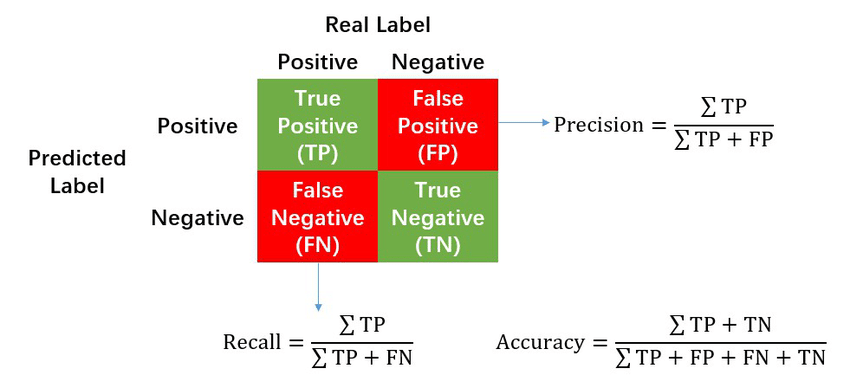
\includegraphics[scale=0.5]{./Figures/precision-recall-accuracy.png}
	\caption{Matriz de confusion \protect\footnotemark.}
	\label{fig:presicion-recall-accuracy}
\end{figure}

\footnotetext{Imagen tomada de \url{https://www.researchgate.net/figure/Calculation-of-Precision-Recall-and-Accuracy-in-the-confusion-matrix_fig3_336402347}}

\subsection{Intersección sobre Unión (IOU)}

La métrica de IOU evalúa la superposición entre la caja delimitadora predicha y la caja delimitadora real de un objeto. Se calcula como el cociente entre el área de intersección y el área de unión de ambas cajas. Esta métrica es fundamental en tareas de detección, ya que un IOU alto indica una buena coincidencia espacial entre la predicción y la referencia, como se puede intuir en la siguiente formula:

\begin{equation}
	\text{IoU} = \frac{\text{Área de Intersección}}{\text{Área de Unión}}
	\label{eq:iou}
\end{equation}

\subsection{\textit{Average Precision} (AP) y \textit{Mean Average Precision} (mAP)}

\begin{itemize}
	\item AP: para cada clase de objeto, se calcula el promedio de la precisión, integrando la curva de precisión-recuperación (ROC). La AP resume el rendimiento del detector en diferentes umbrales de decisión.
	\item mAP: es la media aritmética de la AP calculada para cada clase. El mAP es ampliamente utilizado en competencias y evaluaciones de modelos de detección de objetos, ya que proporciona una única medida que resume la efectividad global del modelo.
\end{itemize}

\subsection{Otras métricas relevantes}

Además de las métricas anteriormente descritas, en la práctica se pueden utilizar otros indicadores, dependiendo de la aplicación y la naturaleza de los datos: \begin{itemize}
	\item Curva ROC y área bajo la curva (AUC): la curva ROC y el AUC se emplean comúnmente en tareas de clasificación para evaluar la capacidad del modelo en discriminar entre clases.
	\item Error Cuadrático Medio (MSE) y Error Absoluto Medio (MAE): en aplicaciones que requieren regresión, como la estimación de posiciones o dimensiones, se utilizan estas métricas para cuantificar la diferencia entre los valores predichos y los reales.
\end{itemize}

La correcta selección y combinación de estas métricas permite una evaluación integral de los modelos de VPC, facilitando tanto la identificación de áreas de mejora como la comparación objetiva entre diferentes enfoques o arquitecturas implementadas.